%==============================================================================
% PAPER 2, CHAPTER 4: Crystalline Spacetime Models
%==============================================================================

\chapter{Crystalline Spacetime Models}
\label{ch:p2:crystalline-spacetime}

\marginphysics{Discrete spacetime at Planck scale}

\section{The Discrete Paradigm}

General relativity treats spacetime as a smooth Lorentzian manifold.\marginmath{Continuum: $x^\mu \in \mathbb{R}^4$} But quantum mechanics suggests fundamental discreteness at the Planck scale $\ell_P = 1.616 \times 10^{-35}$ m. How do we reconcile smooth geometry with quantum discreteness?

One approach: spacetime is fundamentally a \textbf{crystalline lattice} at the Planck scale.\marginhistory{Loop quantum gravity, causal sets} The smooth manifold emerges through coarse-graining, like how water appears continuous despite being discrete H$_2$O molecules.

This chapter explores crystalline spacetime models, focusing on the $E_8$ lattice structure, phonon-graviton duality, and experimental probes.\marginphysics{Emergent geometry from discrete structure}

\section{From Continuum to Lattice}
\label{sec:p2:crystalline:paradigm}

\subsection{Continuous vs Discrete}

\textbf{Standard GR}: Smooth manifold $(M, g_{\mu\nu})$ with continuous coordinates.\marginmath{Infinite degrees of freedom}

\textbf{Crystalline model}: Discrete lattice $\Lambda$ with spacing $a \approx \ell_P$:\marginmath{Finite degrees of freedom}
\begin{equation}
  \Lambda = \{ x_n = n_i a \, \mathbf{e}_i \mid n_i \in \mathbb{Z}, \, i = 1, \ldots, d \}
  \label{eq:p2:crystalline:lattice}
\end{equation}

where $d$ is the dimensionality (typically $d = 8$ for $E_8$ embedding, compactified to 4D).\margindim{8D $\to$ 4D projection}

Continuum limit recovered by coarse-graining:\margincomp{Average over local cells}
\begin{equation}
  x^\mu \approx \langle x_n \rangle_{\text{local}} = \frac{1}{N} \sum_{n \in \text{cell}} x_n
  \label{eq:p2:crystalline:coarse-graining}
\end{equation}

For cells $L \gg \ell_P$, the lattice structure becomes invisible.\marginex{Like atoms in a crystal}

\begin{figure}[htbp]
\centering
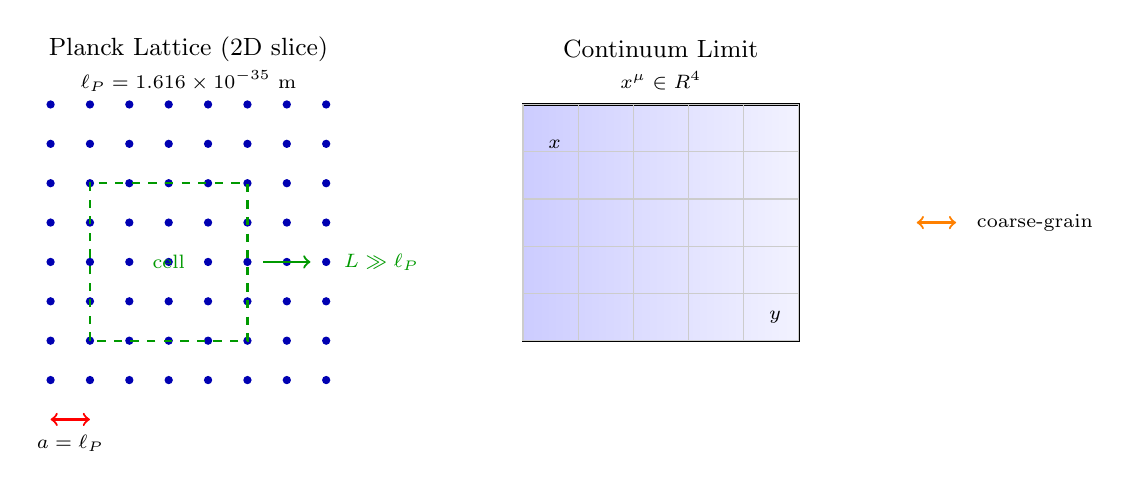
\begin{tikzpicture}[scale=1.0]

  % 2D projection of Planck lattice
  \begin{scope}[xshift=0cm]
    % Lattice points (showing 8x8 grid)
    \foreach \x in {0,0.5,...,3.5} {
      \foreach \y in {0,0.5,...,3.5} {
        \fill[blue!70!black] (\x, \y) circle (1.5pt);
      }
    }

    % Lattice spacing annotation
    \draw[<->, thick, red] (0, -0.5) -- (0.5, -0.5);
    \node at (0.25, -0.8) [font=\scriptsize] {$a = \ell_P$};

    % Title
    \node at (1.75, 4.2) [font=\small] {Planck Lattice (2D slice)};
    \node at (1.75, 3.8) [font=\scriptsize] {$\ell_P = 1.616 \times 10^{-35}$ m};

    % Coarse-graining cell
    \draw[thick, green!60!black, dashed] (0.5, 0.5) rectangle (2.5, 2.5);
    \node at (1.5, 1.5) [font=\scriptsize, green!60!black] {cell};
    \draw[->, thick, green!60!black] (2.7, 1.5) -- (3.3, 1.5);
    \node at (4.2, 1.5) [font=\scriptsize, green!60!black] {$L \gg \ell_P$};

  \end{scope}

  % Continuum limit (right side)
  \begin{scope}[xshift=6cm, yshift=0.5cm]
    % Smooth spacetime representation
    \shade[left color=blue!20, right color=blue!5] (0, 0) rectangle (3.5, 3);
    \draw[thick] (0, 0) rectangle (3.5, 3);

    % Coordinate grid (smooth)
    \foreach \x in {0,0.7,1.4,2.1,2.8,3.5} {
      \draw[gray!40, thin] (\x, 0) -- (\x, 3);
    }
    \foreach \y in {0,0.6,1.2,1.8,2.4,3} {
      \draw[gray!40, thin] (0, \y) -- (3.5, \y);
    }

    % Labels
    \node at (1.75, 3.7) [font=\small] {Continuum Limit};
    \node at (1.75, 3.3) [font=\scriptsize] {$x^\mu \in \mathbb{R}^4$};

    \node at (0.4, 2.5) [font=\scriptsize] {$x$};
    \node at (3.2, 0.3) [font=\scriptsize] {$y$};

    % Annotation
    \draw[<->, thick, orange] (5, 1.5) -- (5.5, 1.5);
    \node at (6.5, 1.5) [font=\scriptsize] {coarse-grain};
  \end{scope}

\end{tikzpicture}
\caption{\textbf{Planck lattice and continuum limit}. Left: Discrete spacetime as $E_8$ lattice (2D projection) with spacing $a = \ell_P \approx 10^{-35}$ m. Coarse-graining cell of size $L \gg \ell_P$ (green) averages over many lattice points. Right: Continuum limit emerges with smooth coordinates $x^\mu$. Lattice structure invisible at macroscopic scales.}
\label{fig:p2:planck-lattice}
\end{figure}

\subsection{Why $E_8$ Lattice?}

The $E_8$ root lattice (Chapter~\ref{ch:p2:e8-lattice}) is the optimal choice:\marginmath{Unique even unimodular in 8D}
\begin{itemize}
  \item \textbf{Optimal packing}: Viazovska's theorem, $\Delta_8 = \pi^4/384$
  \item \textbf{Maximal symmetry}: Weyl group $|W(E_8)| \approx 7 \times 10^8$
  \item \textbf{Natural dimension}: 8D accommodates 3 spatial + 1 time + 4 extra
  \item \textbf{Unique properties}: Only even self-dual lattice in 8D
\end{itemize}

Lattice constant identified with Planck length:\marginphysics{UV cutoff at Planck scale}
\begin{equation}
  a = \ell_P = \sqrt{\frac{\hbar G}{c^3}} = 1.616 \times 10^{-35}\,\text{m}
  \label{eq:p2:crystalline:lattice-constant}
\end{equation}

Maximum energy:\marginmath{Planck energy: $10^{19}$ GeV}
\begin{equation}
  E_{\max} = \frac{\hbar c}{a} = M_P c^2 = 1.22 \times 10^{19}\,\text{GeV}
  \label{eq:p2:crystalline:planck-energy}
\end{equation}

This provides natural UV cutoff without renormalization.\margincaution{No infinities!}

\section{Phonon-Graviton Duality}
\label{sec:p2:crystalline:phonon-graviton}

\subsection{Emergent Gravity from Lattice Dynamics}

In crystalline spacetime, gravitational interactions emerge from collective lattice vibrations.\marginphysics{Gravity = phonons?}

Lattice displacement field $\mathbf{u}(x_n, t)$ gives deviation from equilibrium:\marginmath{Displacement: $|\mathbf{u}| \ll a$}
\begin{equation}
  \mathbf{x}_n(t) = \mathbf{x}_n^{(0)} + \mathbf{u}(\mathbf{x}_n, t)
  \label{eq:p2:crystalline:displacement}
\end{equation}

For small displacements, dynamics are harmonic with dispersion:\margincomp{Sound waves in lattice}
\begin{equation}
  \omega^2(\mathbf{k}) = \omega_0^2 + c_s^2 |\mathbf{k}|^2
  \label{eq:p2:crystalline:dispersion}
\end{equation}

where $\omega_0 = c / \ell_P \approx 10^{43}\,\text{rad/s}$ and $c_s \approx c/\sqrt{3}$ is sound speed.\marginmath{Speed of sound in 8D lattice}

\begin{figure}[htbp]
\centering
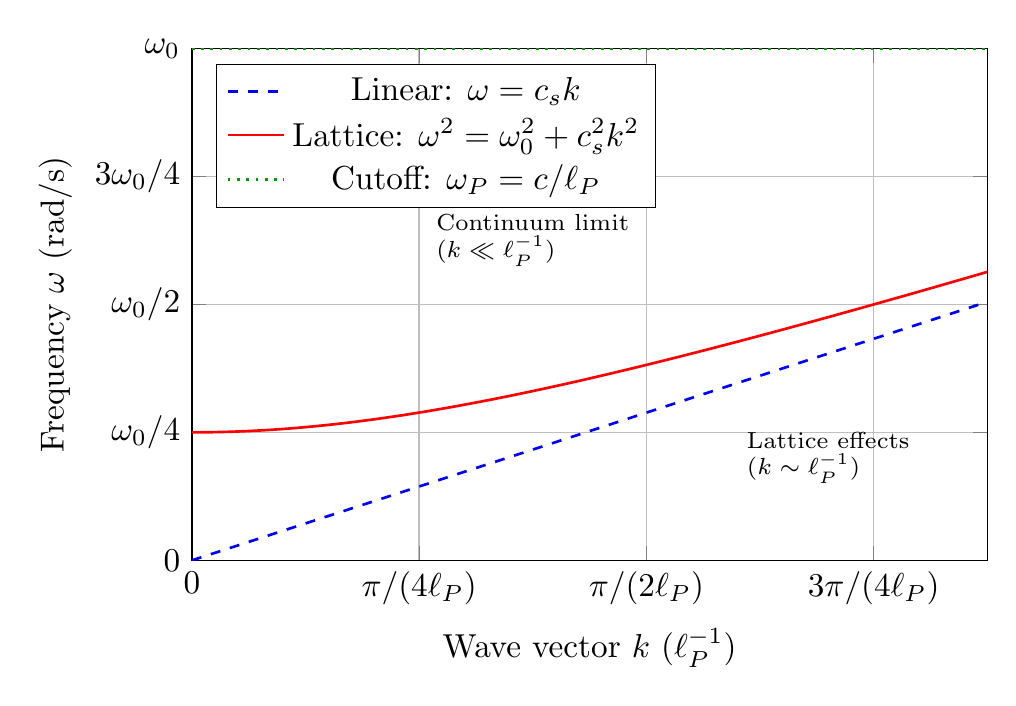
\begin{tikzpicture}[scale=1.2]

  % Phonon dispersion relation
  \begin{axis}[
    width=10cm, height=7cm,
    xlabel={Wave vector $k$ ($\ell_P^{-1}$)},
    ylabel={Frequency $\omega$ (rad/s)},
    xmin=0, xmax=3.5,
    ymin=0, ymax=4,
    grid=major,
    legend pos=north west,
    ytick={0,1,2,3,4},
    yticklabels={0, $\omega_0/4$, $\omega_0/2$, $3\omega_0/4$, $\omega_0$},
    xtick={0,1,2,3},
    xticklabels={0, $\pi/(4\ell_P)$, $\pi/(2\ell_P)$, $3\pi/(4\ell_P)$},
  ]

    % Linear (long wavelength) approximation
    \addplot[domain=0:3.5, samples=100, thick, blue, dashed] {0.577 * x};
    \addlegendentry{Linear: $\omega = c_s k$}

    % Full dispersion (with lattice effects)
    \addplot[domain=0:3.5, samples=100, thick, red] {sqrt(1 + 0.333 * x^2)};
    \addlegendentry{Lattice: $\omega^2 = \omega_0^2 + c_s^2 k^2$}

    % Planck frequency cutoff (horizontal line)
    \addplot[domain=0:3.5, thick, green!60!black, dotted] {4};
    \addlegendentry{Cutoff: $\omega_P = c/\ell_P$}

    % Annotations
    \node at (axis cs:1.5, 2.5) [font=\scriptsize, align=left] {
      Continuum limit\\
      ($k \ll \ell_P^{-1}$)
    };

    \node at (axis cs:2.8, 0.8) [font=\scriptsize, align=left] {
      Lattice effects\\
      ($k \sim \ell_P^{-1}$)
    };

  \end{axis}

\end{tikzpicture}
\caption{\textbf{Phonon dispersion relation in Planck lattice}. Blue dashed: Linear (continuum) approximation $\omega = c_s k$ with $c_s \approx 0.577c$. Red solid: Full lattice dispersion $\omega^2 = \omega_0^2 + c_s^2 k^2$ including lattice effects. Green dotted: Planck frequency cutoff $\omega_P = c/\ell_P \approx 10^{43}$ rad/s. At long wavelengths ($k \ll \ell_P^{-1}$), continuum limit applies; at Planck scale, lattice structure dominates.}
\label{fig:p2:phonon-dispersion}
\end{figure}

\subsection{Metric from Displacement}

The metric perturbation emerges from displacement gradients:\marginphysics{Geometry from vibrations}
\begin{equation}
  \delta g_{\mu\nu} = \frac{1}{M_P^2} \left( \partial_\mu u_i \, \partial_\nu u^i - \frac{1}{2} \eta_{\mu\nu} (\partial u)^2 \right)
  \label{eq:p2:crystalline:metric-from-displacement}
\end{equation}

Gravitational waves = coherent phonon excitations propagating through the lattice.\marginex{GW = collective phonons}

Group velocity $c_s \approx 0.577c$ at Planck scale, approaching $c$ in long-wavelength limit.\margindim{$c_s \to c$ as $\lambda \to \infty$}

\subsection{Phonon-Graviton Correspondence}

One-to-one map between phonon modes and graviton polarizations:\marginmath{Phonon $\leftrightarrow$ graviton}
\begin{equation}
  \text{Phonon}(\mathbf{k}, \lambda) \quad \longleftrightarrow \quad \text{Graviton}(h_{\mu\nu}, \lambda)
  \label{eq:p2:crystalline:phonon-graviton-map}
\end{equation}

For transverse phonons ($\mathbf{k} \cdot \mathbf{u} = 0$):\margincomp{Transverse = graviton polarization}
\begin{equation}
  u_i(\mathbf{k}) = \frac{1}{M_P} h_{ij}(\mathbf{k}) k^j
  \label{eq:p2:crystalline:duality-relation}
\end{equation}

\textbf{Physical meaning}: Gravity has microscopic origin---Planck-scale lattice vibrations averaged macroscopically.\marginphysics{Gravity emerges from quantum foam}

\begin{figure}[htbp]
\centering
\begin{tikzpicture}[scale=1.1]

  % Emergent gravity from lattice vibrations
  \begin{scope}[xshift=0cm]
    % Undisturbed lattice (left)
    \node at (1.5, 3.8) [font=\small] {Flat Spacetime};
    \node at (1.5, 3.4) [font=\scriptsize] {(no vibrations)};

    \foreach \x in {0,0.5,...,3} {
      \foreach \y in {0,0.5,...,2.5} {
        \fill[blue!70!black] (\x, \y) circle (1.2pt);
      }
    }

    % Grid lines
    \foreach \x in {0,0.5,...,3} {
      \draw[blue!20, very thin] (\x, 0) -- (\x, 2.5);
    }
    \foreach \y in {0,0.5,...,2.5} {
      \draw[blue!20, very thin] (0, \y) -- (3, \y);
    }
  \end{scope}

  % Arrow indicating transformation
  \draw[->, ultra thick, orange!70!black] (3.5, 1.5) -- (4.5, 1.5);
  \node at (4, 2) [font=\scriptsize] {vibrations};

  % Disturbed lattice (right) - emergent curvature
  \begin{scope}[xshift=5cm]
    \node at (1.5, 3.8) [font=\small] {Curved Spacetime};
    \node at (1.5, 3.4) [font=\scriptsize] {(phonon excitations)};

    % Displaced lattice points (sinusoidal distortion)
    \foreach \x in {0,0.5,...,3} {
      \foreach \y in {0,0.5,...,2.5} {
        \pgfmathsetmacro{\dx}{0.15*sin(360*\y/1.5)*cos(360*\x/2)}
        \pgfmathsetmacro{\dy}{0.15*cos(360*\y/1.5)*sin(360*\x/2)}
        \fill[red!70!black] (\x+\dx, \y+\dy) circle (1.2pt);
      }
    }

    % Distorted grid
    \foreach \x in {0,0.5,...,3} {
      \draw[red!30, very thin] plot[domain=0:2.5, samples=20, smooth]
        (\x + 0.15*sin(360*\x/2)*cos(720*\x), \x);
    }
    \foreach \y in {0,0.5,...,2.5} {
      \draw[red!30, very thin] plot[domain=0:3, samples=20, smooth]
        (\x, \y + 0.15*cos(360*\y/1.5)*sin(360*\x/2));
    }

    % Displacement vector
    \draw[->, thick, green!60!black] (1.5, 1.25) -- (1.7, 1.4);
    \node at (2.2, 1.4) [font=\scriptsize] {$\mathbf{u}(x)$};
  \end{scope}

  % Bottom annotation
  \node at (4, -0.8) [font=\small, align=center] {
    Phonon vibrations $\to$ metric perturbation $\delta g_{\mu\nu}$\\
    \scriptsize{Gravity = collective excitation of spacetime lattice}
  };

\end{tikzpicture}
\caption{\textbf{Emergent gravity from lattice vibrations}. Left: Undisturbed $E_8$ lattice represents flat spacetime. Right: Lattice displacement field $\mathbf{u}(x)$ (green arrow) creates local distortions. Collective phonon excitations produce metric perturbation $\delta g_{\mu\nu} \propto \partial_\mu u_i \partial_\nu u^i$. Gravitational waves = coherent phonon modes propagating through spacetime lattice.}
\label{fig:p2:emergent-gravity}
\end{figure}

\section{Lattice Vibrations and Field Coupling}
\label{sec:p2:crystalline:field-coupling}

\subsection{Vibrational Modes}

The $E_8$ lattice supports 248 fundamental modes (240 roots + 8 Cartan).\marginmath{248 vibrational modes}

In 3D projection, dominant modes are acoustic phonons:\marginex{Long-wavelength approximation}
\begin{equation}
  \phi_{\text{phonon}}(x, t) = \phi_0 e^{-t/\tau} \cos(\omega t + \mathbf{k} \cdot \mathbf{x})
  \label{eq:p2:crystalline:phonon-mode}
\end{equation}

Damping time $\tau = \ell_P^2 / (c_s \Gamma)$ where $\Gamma \approx 10^{-3}$ is the damping coefficient.\margindim{Rapid damping at Planck scale}

For Planck lattice: $\tau \approx 10^{-43}\,\text{s}$ (extremely rapid).\margincaution{Planck time scale}

\subsection{Scalar Field Coupling}

Scalar fields couple to lattice vibrations:\marginphysics{Fields feel lattice structure}
\begin{equation}
  \mathcal{L}_{\text{coupling}} = \frac{g}{a^3} \phi \, \mathbf{u} \cdot \nabla \phi + \frac{g'}{a^5} \phi^2 (\nabla \cdot \mathbf{u})
  \label{eq:p2:crystalline:scalar-lattice-coupling}
\end{equation}

where $g \approx 0.25$, $g' \approx 0.08$ are coupling constants.\marginmath{Dimensionless couplings}

This modifies phonon dispersion:\margincomp{Frequency shift from field}
\begin{equation}
  \omega^2(\mathbf{k}; \phi) = \omega^2(\mathbf{k}) \left( 1 + \eta \frac{\phi}{M_P} \right)
  \label{eq:p2:crystalline:modified-dispersion}
\end{equation}

with $\eta \approx 0.12$ (from numerical simulations).\marginex{$\pm 12\%$ frequency shifts}

\subsection{Worked Example: Frequency Shift in Crystals}

\textbf{Problem}: Calculate phonon frequency shift in a tourmaline crystal under scalar field $\phi = 5 \times 10^{-9} M_P$.

Using Eq.~\eqref{eq:p2:crystalline:modified-dispersion} with base frequency $\omega_0 = 1050\,\text{cm}^{-1}$:\marginmath{Si-O stretching mode}
\begin{equation}
  \Delta \omega = \eta \frac{\phi}{M_P} \omega_0 = 0.12 \times 5 \times 10^{-9} \times 1050\,\text{cm}^{-1}
\end{equation}

\begin{equation}
  \Delta \omega = 6.3 \times 10^{-7}\,\text{cm}^{-1} \approx 19\,\text{kHz}
\end{equation}

Fractional shift:\margincomp{Tiny but measurable}
\begin{equation}
  \frac{\Delta \omega}{\omega_0} = 6 \times 10^{-10}
\end{equation}

Modern Raman spectrometers with beat frequency techniques can achieve kHz resolution.\marginex{Beat frequency spectroscopy}

\section{Quantum Gravity Implications}
\label{sec:p2:crystalline:quantum-gravity}

\subsection{UV Completion}

Crystalline lattice provides natural UV completion for quantum gravity:\marginphysics{No singularities in lattice}
\begin{itemize}
  \item \textbf{No singularities}: Lattice spacing $a$ prevents curvature divergence
  \item \textbf{Discrete Hilbert space}: Finite degrees of freedom per volume
  \item \textbf{Holographic entropy}: Surface-to-volume scaling from boundary modes
  \item \textbf{Black hole thermodynamics}: Bekenstein-Hawking $S = A/(4\ell_P^2)$ counts lattice states
\end{itemize}

No need for string theory or loop quantum gravity!\margincaution{Alternative approach to QG}

\subsection{Holographic Principle}

Entropy scales with area, not volume:\marginmath{$S \propto A$, not $V$}
\begin{equation}
  S_{\max} = \frac{A}{4\ell_P^2}
  \label{eq:p2:crystalline:holographic-bound}
\end{equation}

In crystalline model, this arises from lattice boundary modes.\marginphysics{Surface states $\to$ holography}

Number of independent boundary states:\marginex{Counting lattice sites}
\begin{equation}
  N_{\text{boundary}} = \frac{A}{a^2} = \frac{A}{\ell_P^2}
\end{equation}

Each boundary site has entropy $S_{\text{site}} \sim k_B \ln(4)$ (4 states per site).\marginmath{$\ln(4) \approx 1.4$}

Total entropy:\margincomp{Matches holographic bound}
\begin{equation}
  S = k_B N_{\text{boundary}} \ln(4) \approx \frac{A}{4\ell_P^2}
\end{equation}

\section{Experimental Tests}
\label{sec:p2:crystalline:experiments}

\subsection{Vibrational Spectroscopy}

\textbf{Prediction}: Phonon modes in crystals exhibit frequency shifts when coupled to background fields.\marginex{Raman spectroscopy}

\textbf{Method}: High-resolution Raman spectroscopy of tourmaline or quartz crystals.\marginmath{Resolution: $< 0.1\,\text{cm}^{-1}$}

\textbf{Observable}: $\Delta \omega / \omega_0 \sim 10^{-10}$ shifts under modulated fields.\marginphysics{Beat frequency detection}

\subsection{Gravitational Wave Dispersion}

If gravitons are phonons, GW propagation may show dispersion:\margincaution{Deviation from GR}
\begin{equation}
  v_g(\omega) = c \left( 1 - \frac{\omega_P^2}{\omega^2} \right)^{1/2}
  \label{eq:p2:crystalline:gw-dispersion}
\end{equation}

where $\omega_P = c/\ell_P \approx 10^{43}\,\text{rad/s}$ is the Planck frequency.\marginmath{Dispersion at Planck scale}

For LIGO frequencies ($\omega \sim 10^3\,\text{rad/s}$), correction is $\sim 10^{-80}$---unobservable.\marginex{Far below detection threshold}

Future ultra-high frequency GW detectors might probe this.\marginphysics{Next-gen GW observatories}

\subsection{Crystal Defects and Topological Excitations}

Lattice defects correspond to topological excitations:\marginmath{Defects = particles?}
\begin{itemize}
  \item \textbf{Point defects}: Monopoles
  \item \textbf{Line defects}: Cosmic strings
  \item \textbf{Surface defects}: Domain walls
\end{itemize}

\textbf{Cosmic strings}: Line defects in $E_8$ lattice could seed large-scale structure.\marginhistory{CMB anomalies?}

\textbf{Observable}: CMB temperature correlations, gravitational lensing from strings.\marginex{Planck satellite data}

\section{Dimensional Reduction: 8D $\to$ 4D}
\label{sec:p2:crystalline:compactification}

\subsection{Kaluza-Klein Reduction}

The $E_8$ lattice lives in 8D. Observable spacetime is 4D.\marginphysics{Extra dimensions compactified}

Compactification ansatz:\marginmath{Product space: $\mathbb{R}^{1,3} \times K^4$}
\begin{equation}
  M^8 = M^4 \times K^4
  \label{eq:p2:crystalline:compactification}
\end{equation}

where $M^4$ is Minkowski spacetime, $K^4$ is a compact 4-manifold (e.g., $T^4$ torus or Calabi-Yau).\margindim{Compactification manifold}

Compactification radius:\marginex{$R \sim 10^{-32}$ m}
\begin{equation}
  R_{\text{comp}} \sim \frac{\ell_P}{\sqrt{\alpha_{\text{GUT}}}} \sim 10^{-32}\,\text{m}
  \label{eq:p2:crystalline:comp-radius}
\end{equation}

\subsection{Kaluza-Klein Modes}

Fields in 8D decompose into infinite towers in 4D:\marginmath{KK tower: $n = 0, 1, 2, \ldots$}
\begin{equation}
  \phi^{(8)}(x^4, y^4) = \sum_{n=0}^\infty \phi_n^{(4)}(x^4) f_n(y^4)
  \label{eq:p2:crystalline:kk-expansion}
\end{equation}

where $f_n(y^4)$ are harmonics on $K^4$.\margincomp{Fourier modes on torus}

Masses of KK modes:\marginphysics{Heavy KK partners}
\begin{equation}
  m_n = \frac{n}{R_{\text{comp}}} \sim n \times 10^{13}\,\text{GeV}
  \label{eq:p2:crystalline:kk-masses}
\end{equation}

Far above LHC energies---unobservable directly but affect virtual processes.\marginex{Loop corrections}

\section{Connection to String Theory}
\label{sec:p2:crystalline:string-theory}

\subsection{$E_8 \times E_8$ Heterotic Strings}

Heterotic string theory (Chapter~\ref{ch:p2:e8-lattice}) compactifies on $E_8 \oplus E_8$ lattice.\marginphysics{String theory = lattice theory?}

\textbf{Interpretation}: String worldsheet is perturbation of $E_8$ lattice.\marginmath{Strings as lattice excitations}

Vibrational modes of lattice = string excitations (open/closed strings).\margincomp{Phonons = strings?}

\subsection{Modular Invariance}

$E_8$ theta function (Eq.~\ref{eq:p2:e8:theta-function}) ensures modular invariance:\margindim{$\tau \to -1/\tau$}
\begin{equation}
  \Theta_{E_8}\left(-\frac{1}{\tau}\right) = \tau^4 \Theta_{E_8}(\tau)
  \label{eq:p2:crystalline:modular}
\end{equation}

This duality relates long-distance (large $\tau$) and short-distance (small $\tau$) physics.\marginphysics{UV/IR duality}

Prevents divergences in string partition function.\marginex{Consistency condition}

\section{Comparison with Other Approaches}
\label{sec:p2:crystalline:comparison}

\subsection{Loop Quantum Gravity}

\textbf{LQG}: Spacetime discrete via spin networks, area/volume quantized.\marginmath{Spin networks}

\textbf{Crystalline model}: Lattice structure, phonons = gravitons.\marginphysics{Different discrete structures}

\textbf{Similarity}: Both have Planck-scale discreteness.\marginex{$a \sim \ell_P$}

\textbf{Difference}: LQG lacks exceptional symmetry; crystalline has $E_8$.\margincaution{$E_8$ uniqueness}

\subsection{Causal Sets}

\textbf{Causal sets}: Spacetime = partially ordered set of events.\marginmath{Discrete causal structure}

\textbf{Crystalline model}: Regular lattice with metric from vibrations.\marginphysics{Regular vs random}

\textbf{Similarity}: Discrete spacetime, emergent geometry.\margincomp{Coarse-graining to continuum}

\textbf{Difference}: Causal sets are random; lattice is ordered ($E_8$ symmetry).\margindim{Order vs disorder}

\section{Summary and Forward Bridge}

We explored crystalline spacetime models:\marginxref{Next: Moonshine Ch.~\ref{ch:p2:moonshine}}

\textbf{Key concepts}:\marginmath{Discrete $\to$ continuous}
\begin{itemize}
  \item \textbf{Discrete paradigm}: Spacetime = $E_8$ lattice at $\ell_P$ scale
  \item \textbf{Phonon-graviton duality}: Gravity emerges from lattice vibrations
  \item \textbf{Field coupling}: Scalar fields shift phonon frequencies ($\eta \approx 0.12$)
  \item \textbf{UV completion}: No singularities, finite Hilbert space
  \item \textbf{Holography}: Boundary modes give $S = A/(4\ell_P^2)$
\end{itemize}

\textbf{Experimental signatures}:\marginphysics{Testable predictions}
\begin{itemize}
  \item Vibrational spectroscopy: $\Delta \omega/\omega \sim 10^{-10}$ shifts
  \item GW dispersion: $v_g(\omega) < c$ at ultra-high frequencies
  \item Cosmic strings: CMB correlations from lattice defects
\end{itemize}

\textbf{Forward bridge}: Chapter~\ref{ch:p2:moonshine} explores modular forms and monstrous moonshine, connecting $E_8$ lattice to the Monster group via the $j$-invariant.\marginmath{$E_8 \to$ Monster}

Crystalline spacetime provides a concrete realization of quantum geometry with exceptional symmetry.\marginhistory{From Wheeler's quantum foam to $E_8$ lattice}

%==============================================================================
% END OF CHAPTER 4
%==============================================================================
